\protect\hyperlink{main-nav}{≡} \protect\hyperlink{close-nav}{×}

\hypertarget{section-2.6-second-derivative-and-concavity}{%
\section{Section 2.6: Second Derivative and
Concavity}\label{section-2.6-second-derivative-and-concavity}}

\hypertarget{second-derivative-and-concavity}{%
\subsection{Second Derivative and
Concavity}\label{second-derivative-and-concavity}}

Graphically, a function is \textbf{concave up} if its graph is curved
with the opening upward (Figure 1a). Similarly, a function is
\textbf{concave down} if its graph opens downward (Figure 1b).

\begin{figure}
\centering
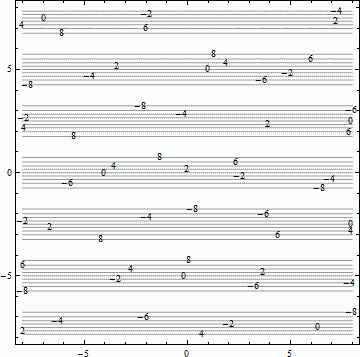
\includegraphics{images/image044.png}
\caption{Figure 1}
\end{figure}

This figure shows the concavity of a function at several points. Notice
that a function can be concave up regardless of whether it is increasing
or decreasing.

\begin{figure}
\centering
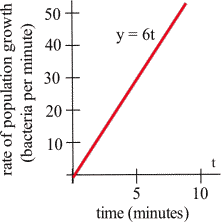
\includegraphics{images/image045.png}
\caption{}
\end{figure}

For example, \textbf{an epidemic}: Suppose an epidemic has started, and
you, as a member of congress, must decide whether the current methods
are effectively fighting the spread of the disease or whether more
drastic measures and more money are needed. In Figure 2 below,
\textbackslash{}(f(x)\textbackslash{}) is the number of people who have
the disease at time \textbackslash{}(x\textbackslash{}), and two
different situations are shown. In both Figure 2a and Figure 2b, the
number of people with the disease,
\textbackslash{}(f(\textbackslash{}text\{now\})\textbackslash{}), and
the rate at which new people are getting sick,
\textbackslash{}(f'(\textbackslash{}text\{now\})\textbackslash{}), are
the same. The difference in the two situations is the concavity of
\textbackslash{}(f\textbackslash{}), and that difference in concavity
might have a big effect on your decision.

\begin{figure}
\centering
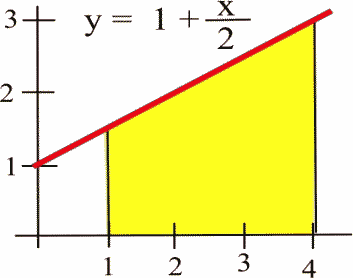
\includegraphics{images/image046.png}
\caption{Figure 2}
\end{figure}

In Figure 2a, \textbackslash{}(f\textbackslash{}) is concave down at
"now", the slopes are decreasing, and it looks as if it is tailing off.
We can say "\textbackslash{}(f\textbackslash{}) is increasing at a
decreasing rate." It appears that the current methods are starting to
bring the epidemic under control.

In Figure 2b, \textbackslash{}(f\textbackslash{}) is concave up, the
slopes are increasing, and it looks as if it will keep increasing faster
and faster. It appears that the epidemic is still out of control.

The differences between the graphs come from whether the
\emph{derivative} is increasing or decreasing

The derivative of a function f is a function that gives information
about the slope of \textbackslash{}(f\textbackslash{}). \textbf{The
derivative tells us if the original function is increasing or
decreasing}.

Because \textbackslash{}(f'\textbackslash{}) is a function, we can take
its derivative. This second derivative also gives us information about
our original function \textbackslash{}(f\textbackslash{}). The second
derivative gives us a mathematical way to tell how the graph of a
function is curved. \textbf{The second derivative tells us if the
original function is concave up or down}.

To view this video please enable JavaScript, and consider upgrading to a
web browser that \href{http://videojs.com/html5-video-support/}{supports
HTML5 video}

\hypertarget{second-derivative}{%
\paragraph{Second Derivative}\label{second-derivative}}

Let \textbackslash{}( y=f(x) \textbackslash{}). The \textbf{second
derivative of \textbackslash{}(f\textbackslash{})} is the derivative of
\textbackslash{}( y'=f'(x) \textbackslash{}).

Using prime notation, this is \textbackslash{}( f''(x) \textbackslash{})
or \textbackslash{}( y'' \textbackslash{}). You can read this aloud as
"f double prime of x" or "y double prime."

Using Leibniz notation, the second derivative is written
\textbackslash{}( \textbackslash{}frac\{d\^{}2y\}\{dx\^{}2\}
\textbackslash{}) or \textbackslash{}(
\textbackslash{}frac\{d\^{}2f\}\{dx\^{}2\} \textbackslash{}). This is
read aloud as "the second derivative of y (or f)."

If \textbackslash{}( f''(x) \textbackslash{}) is positive on an
interval, the graph of \textbackslash{}( y=f(x) \textbackslash{}) is
\textbf{concave up} on that interval. We can say that
\textbackslash{}(f\textbackslash{}) is increasing (or decreasing)
\textbf{at an increasing rate}.

If \textbackslash{}( f''(x) \textbackslash{}) is negative on an
interval, the graph of \textbackslash{}( y=f(x) \textbackslash{}) is
\textbf{concave down} on that interval. We can say that
\textbackslash{}(f\textbackslash{}) is increasing (or decreasing)
\textbf{at a decreasing rate}.

\hypertarget{example-1}{%
\paragraph{Example 1}\label{example-1}}

Find \textbackslash{}( f''(x) \textbackslash{}) for \textbackslash{}(
f(x)=3x\^{}7 \textbackslash{}).

First, we need to find the first derivative:
\textbackslash{}{[}f'(x)=21x\^{}6.\textbackslash{}{]}

Then we take the derivative of that function:
\textbackslash{}{[}f''(x)=\textbackslash{}frac\{d\}\{dx\}\textbackslash{}left(
f'(x)
\textbackslash{}right)=\textbackslash{}frac\{d\}\{dx\}\textbackslash{}left(
21x\^{}6 \textbackslash{}right)=126x\^{}5. \textbackslash{}{]}

If \textbackslash{}(f(x)\textbackslash{}) represents the position of a
particle at time \textbackslash{}(x\textbackslash{}), then
\textbackslash{}(v(x) = f '(x)\textbackslash{}) will represent the
velocity (rate of change of the position) of the particle and
\textbackslash{}(a(x) = v '(x) = f ''(x)\textbackslash{}) will represent
the acceleration (the rate of change of the velocity) of the particle.

You are probably familiar with acceleration from driving or riding in a
car. The speedometer tells you your velocity (speed). When you leave
from a stop and press down on the accelerator, you are accelerating --
increasing your speed.

\hypertarget{example-2}{%
\paragraph{Example 2}\label{example-2}}

The height (feet) of a particle at time
\textbackslash{}(t\textbackslash{}) seconds is \textbackslash{}(f(t) =
t\^{}3 -- 4t\^{}2 + 8t\textbackslash{}). Find the height, velocity and
acceleration of the particle when \textbackslash{}(t =\textbackslash{})
0, 1, and 2 seconds.

\textbackslash{}(f(t) = t\^{}3 -- 4t\^{}2 + 8t\textbackslash{}) so
\textbackslash{}(f(0) = 0\textbackslash{}) feet, \textbackslash{}(f(1) =
5\textbackslash{}) feet, and \textbackslash{}(f(2) = 8\textbackslash{})
feet.

The velocity is \textbackslash{}(v(t) = f '(t) = 3t\^{}2 -- 8t +
8\textbackslash{}) so \textbackslash{}( v(0) = 8\textbackslash{}) ft/s,
\textbackslash{}(v(1) = 3\textbackslash{}) ft/s, and
\textbackslash{}(v(2) = 4\textbackslash{}) ft/s. At each of these times
the velocity is positive and the particle is moving upward, increasing
in height.

The acceleration is \textbackslash{}(a(t) = f ''(t) = 6t --
8\textbackslash{}) so \textbackslash{}(a(0) = --8 \textbackslash{}text\{
ft/s\textbackslash{}(\^{}2\textbackslash{})\}\textbackslash{}),
\textbackslash{}(a(1) = --2 \textbackslash{}text\{
ft/s\textbackslash{}(\^{}2\textbackslash{})\}\textbackslash{}) and
\textbackslash{}(a(2) = 4 \textbackslash{}text\{
ft/s\textbackslash{}(\^{}2\textbackslash{})\}\textbackslash{}).

At time 0 and 1, the acceleration is negative, so the particle's
velocity would be decreasing at those points - the particle was slowing
down. At time 2, the velocity is positive, so the particle was
increasing in speed.

To view this video please enable JavaScript, and consider upgrading to a
web browser that \href{http://videojs.com/html5-video-support/}{supports
HTML5 video}

\hypertarget{inflection-points}{%
\subsection{Inflection Points}\label{inflection-points}}

\hypertarget{definition-inflection-point}{%
\paragraph{Definition (Inflection
Point)}\label{definition-inflection-point}}

An \textbf{inflection point} is a point on the graph of a function where
the concavity of the function changes, from concave up to down or from
concave down to up.

\hypertarget{example-3}{%
\paragraph{Example 3}\label{example-3}}

Which of the labeled points in the graph below are inflection points?

\begin{figure}
\centering
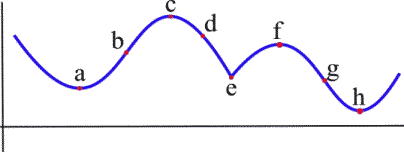
\includegraphics{images/image047.png}
\caption{}
\end{figure}

The concavity changes at points b and g. At points a and h, the graph is
concave up on both sides, so the concavity does not change. At points c
and f, the graph is concave down on both sides. At point e, even though
the graph looks strange there, the graph is concave down on both sides
-- the concavity does not change.

Inflection points happen when the concavity changes. Because we know the
connection between the concavity of a function and the sign of its
second derivative, we can use this to find inflection points.

\hypertarget{working-definition}{%
\paragraph{Working Definition}\label{working-definition}}

An \textbf{inflection point} is a point on the graph where the second
derivative changes sign.

In order for the second derivative to change signs, it must either be
zero or be undefined. So to find the inflection points of a function we
only need to check the points where \textbackslash{}(f
''(x)\textbackslash{}) is 0 or undefined.

Note that it is not enough for the second derivative to be zero or
undefined. We still need to check that the sign of \textbackslash{}( f''
\textbackslash{}) changes sign. The functions in the next example
illustrate what can happen.

\hypertarget{example-4}{%
\paragraph{Example 4}\label{example-4}}

Let \textbackslash{}(f(x) = x\^{}3\textbackslash{}),
\textbackslash{}(g(x) = x\^{}4\textbackslash{}) and
\textbackslash{}(h(x) = x\^{}\{1/3\}\textbackslash{}). For which of
these functions is the point (0,0) an inflection point?

\begin{figure}
\centering
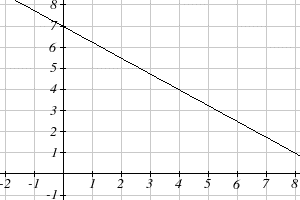
\includegraphics{images/image048.png}
\caption{}
\end{figure}

Graphically, it is clear that the concavity of \textbackslash{}(f(x) =
x\^{}3\textbackslash{}) and \textbackslash{}(h(x) =
x\^{}\{1/3\}\textbackslash{}) changes at (0,0), so (0,0) is an
inflection point for \textbackslash{}(f\textbackslash{}) and
\textbackslash{}(h\textbackslash{}). The function \textbackslash{}(g(x)
= x\^{}4\textbackslash{}) is concave up everywhere so (0,0) is not an
inflection point of \textbackslash{}(g\textbackslash{}).

We can also compute the second derivatives and check the sign change.

If \textbackslash{}(f(x) = x\^{}3\textbackslash{}), then
\textbackslash{}(f'(x) = 3x\^{}2\textbackslash{}) and \textbackslash{}(
f''(x) = 6x\textbackslash{}). The only point at which
\textbackslash{}(f''(x) = 0\textbackslash{}) or is undefined
(\textbackslash{}(f'\textbackslash{}) is not differentiable) is at
\textbackslash{}(x = 0\textbackslash{}). If \textbackslash{}( x
\textbackslash{}lt 0\textbackslash{}), then \textbackslash{}(f ''(x)
\textbackslash{}lt 0\textbackslash{}) so
\textbackslash{}(f\textbackslash{}) is concave down. If
\textbackslash{}(x \textbackslash{}gt 0\textbackslash{}), then
\textbackslash{}(f''(x) \textbackslash{}gt 0\textbackslash{}) so
\textbackslash{}(f\textbackslash{}) is concave up. At \textbackslash{}(x
= 0\textbackslash{}) the concavity changes so the point
\textbackslash{}((0,f(0)) = (0,0)\textbackslash{}) is an inflection
point of \textbackslash{}(f(x)=x\^{}3\textbackslash{}).

If \textbackslash{}(g(x) = x\^{}4\textbackslash{}), then
\textbackslash{}(g'(x) = 4x\^{}3\textbackslash{}) and
\textbackslash{}(g''(x) = 12x\^{}2\textbackslash{}). The only point at
which \textbackslash{}(g''(x) = 0\textbackslash{}) or is undefined is at
\textbackslash{}(x = 0\textbackslash{}). If \textbackslash{}(x
\textbackslash{}lt 0\textbackslash{}), then \textbackslash{}(g''(x)
\textbackslash{}gt 0\textbackslash{}) so
\textbackslash{}(g\textbackslash{}) is concave up. If \textbackslash{}(x
\textbackslash{}gt 0\textbackslash{}), then \textbackslash{}(g ''(x)
\textbackslash{}gt 0\textbackslash{}) so
\textbackslash{}(g\textbackslash{}) is also concave up. At
\textbackslash{}(x = 0\textbackslash{}) the concavity \textbf{does not
change} so the point \textbackslash{}((0, g(0)) = (0,0)\textbackslash{})
is \textbf{not an inflection point} of
\textbackslash{}(g(x)=x\^{}4\textbackslash{}). Keep this example in
mind!

If \textbackslash{}(h(x) = x\^{}\{1/3\}\textbackslash{}), then
\textbackslash{}(h'(x) =
\textbackslash{}frac\{1\}\{3\}x\^{}\{-2/3\}\textbackslash{}) and
\textbackslash{}(h''(x) =
-\textbackslash{}frac\{2\}\{9\}x\^{}\{-5/3\}\textbackslash{}).
\textbackslash{}(h''\textbackslash{}) is not defined if
\textbackslash{}(x = 0\textbackslash{}), but
\textbackslash{}(h''(\textbackslash{}text\{negative number\})
\textbackslash{}gt 0\textbackslash{}) and
\textbackslash{}(h''(\textbackslash{}text\{positive number\})
\textbackslash{}lt 0\textbackslash{}) so
\textbackslash{}(h\textbackslash{}) changes concavity at (0,0) and (0,0)
is an inflection point of \textbackslash{}(h\textbackslash{}).

To view this video please enable JavaScript, and consider upgrading to a
web browser that \href{http://videojs.com/html5-video-support/}{supports
HTML5 video}

\hypertarget{example-5}{%
\paragraph{Example 5}\label{example-5}}

Sketch the graph of a function with \textbackslash{}(f(2) =
3\textbackslash{}), \textbackslash{}(f '(2) = 1\textbackslash{}), and an
inflection point at (2,3).

Two possible solutions are shown here.

\begin{figure}
\centering
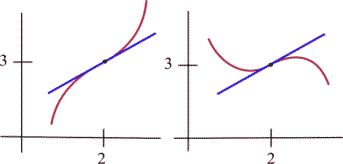
\includegraphics{images/image049.png}
\caption{}
\end{figure}

\begin{longtable}[]{@{}ll@{}}
\toprule
\endhead
\href{section2-5.php}{← Previous Section} & \href{section2-7.php}{Next
Section →}\tabularnewline
\bottomrule
\end{longtable}
